%% ============================================================
%% Paper04_COVID_Corruption_Short.tex
%% Public summary presentation (7 slides)
%% The Effect of the COVID-19 Pandemic on Risk of Corruption
%% Silverio-Murillo, Prudencio & Balmori-de-la-Miyar
%% Public Organization Review (2024)
%%
%% Compile: cd Slides
%%   TEXINPUTS=../Preambles:$TEXINPUTS xelatex -interaction=nonstopmode Paper04_COVID_Corruption_Short.tex
%%   BIBINPUTS=..:$BIBINPUTS bibtex Paper04_COVID_Corruption_Short
%%   TEXINPUTS=../Preambles:$TEXINPUTS xelatex -interaction=nonstopmode Paper04_COVID_Corruption_Short.tex
%%   TEXINPUTS=../Preambles:$TEXINPUTS xelatex -interaction=nonstopmode Paper04_COVID_Corruption_Short.tex
%% ============================================================
\documentclass[aspectratio=169, 10pt]{beamer}
%% ============================================================
%% header.tex -- Shared Beamer preamble for Research Portfolio
%% Compile with: XeLaTeX (3-pass + bibtex)
%% Colors match Quarto/emory-clean.scss for cross-format consistency
%% ============================================================

%% ---- Packages -----------------------------------------------
\usepackage{fontspec}           % XeLaTeX font loading
\usepackage{unicode-math}       % Unicode math support
\usepackage{amsmath, mathtools} % Math environments
\usepackage{booktabs}           % Publication-quality tables
\usepackage{multirow}           % Multi-row table cells
\usepackage{graphicx}           % Include figures
\usepackage{xcolor}             % Color definitions
\usepackage{tcolorbox}          % Colored boxes
\tcbuselibrary{skins, breakable}
\usepackage{natbib}             % Author-year citations
\usepackage{appendixnumberbeamer} % Appendix slides don't count in total
\usepackage{hyperref}           % Hyperlinks
\usepackage{tikz}               % Diagrams (if needed)

%% ---- Fonts --------------------------------------------------
%% Using TeX Gyre Heros (Helvetica-style, bundled with MiKTeX).
%% To switch to Source Sans Pro: install it, then swap the two blocks below.
\setmainfont{TeX Gyre Heros}
\setsansfont{TeX Gyre Heros}
% Alternative: uncomment below and comment above if Source Sans Pro is installed
% \setmainfont{Source Sans Pro}[BoldFont=Source Sans Pro SemiBold]
% \setsansfont{Source Sans Pro}[BoldFont=Source Sans Pro SemiBold]

%% ---- Colors (matching emory-clean.scss) ---------------------
\definecolor{navyblue}{HTML}{012169}
\definecolor{institutgold}{HTML}{2E75B6}   % steel blue (was gold #B9975B)
\definecolor{highlightyellow}{HTML}{F2A900}
\definecolor{lightbg}{HTML}{E8EDF5}
\definecolor{darkgray}{HTML}{1a1a1a}
\definecolor{medgray}{HTML}{555555}
\definecolor{lightgray}{HTML}{f8f9fa}
\definecolor{positivegreen}{HTML}{15803d}
\definecolor{negativered}{HTML}{b91c1c}

%% ---- Beamer Theme -------------------------------------------
\usetheme{default}
\usecolortheme{default}
\setbeamertemplate{navigation symbols}{}   % No navigation clutter

%% Frame title
\setbeamercolor{frametitle}{fg=white, bg=navyblue}
\setbeamertemplate{frametitle}{%
  \vspace*{0.3em}%
  \insertframetitle%
  \vspace*{0.3em}%
}
\setbeamerfont{frametitle}{series=\bfseries, size=\large}

%% Title page colors
\setbeamercolor{title}{fg=navyblue}
\setbeamercolor{subtitle}{fg=institutgold}
\setbeamercolor{author}{fg=navyblue}
\setbeamercolor{institute}{fg=medgray}
\setbeamercolor{date}{fg=institutgold}

%% Body
\setbeamercolor{background canvas}{bg=white}
\setbeamercolor{normal text}{fg=darkgray}
\setbeamerfont{normal text}{family=\sffamily}

%% Itemize bullets
\setbeamercolor{item}{fg=navyblue}
\setbeamercolor{subitem}{fg=institutgold}
\setbeamertemplate{itemize item}{\small\textbullet}
\setbeamertemplate{itemize subitem}{\small$\rightarrow$}

%% Block environments
\setbeamercolor{block title}{fg=white, bg=navyblue}
\setbeamercolor{block body}{fg=darkgray, bg=lightbg}
\setbeamercolor{block title alerted}{fg=white, bg=institutgold}
\setbeamercolor{block body alerted}{fg=darkgray, bg=white}

%% Footer
\setbeamertemplate{footline}{%
  \hfill%
  \usebeamerfont{page number in head/foot}%
  \usebeamercolor[fg]{page number in head/foot}%
  \insertframenumber\,/\,\inserttotalframenumber\kern1em%
  \vskip4pt%
}
\setbeamercolor{page number in head/foot}{fg=medgray}

%% Section slides (automatically centered, navy bg)
\AtBeginSection[]{%
  \begin{frame}[plain]
    \begin{tikzpicture}[remember picture, overlay]
      \fill[navyblue] (current page.south west) rectangle (current page.north east);
      \node[white, font=\bfseries\Large, align=center] at (current page.center)
        {\insertsectionhead};
    \end{tikzpicture}
  \end{frame}%
}

%% ---- Custom Box Environments --------------------------------

%% keybox: gold background, for key takeaways
\newtcolorbox{keybox}{%
  colback=institutgold!12!white,
  colframe=institutgold,
  leftrule=4pt, rightrule=0pt, toprule=0pt, bottomrule=0pt,
  arc=4pt, outer arc=4pt,
  boxsep=2pt, left=6pt, right=6pt, top=5pt, bottom=5pt,
}

%% methodbox: navy left bar, for model/identification
\newtcolorbox{methodbox}{%
  colback=navyblue!5!white,
  colframe=navyblue,
  leftrule=4pt, rightrule=0pt, toprule=0pt, bottomrule=0pt,
  arc=4pt, outer arc=4pt,
  boxsep=2pt, left=6pt, right=6pt, top=5pt, bottom=5pt,
}

%% resultbox: gold border, for main findings
\newtcolorbox{resultbox}{%
  colback=institutgold!10!white,
  colframe=institutgold,
  leftrule=2pt, rightrule=2pt, toprule=2pt, bottomrule=2pt,
  arc=4pt, outer arc=4pt,
  boxsep=2pt, left=6pt, right=6pt, top=5pt, bottom=5pt,
}

%% assumptionbox: titled, formal assumptions
\newtcolorbox{assumptionbox}[1][]{%
  colback=highlightyellow!8!white,
  colframe=highlightyellow!70!black,
  leftrule=2pt, rightrule=2pt, toprule=2pt, bottomrule=2pt,
  arc=4pt, outer arc=4pt,
  boxsep=2pt, left=6pt, right=6pt, top=5pt, bottom=5pt,
  title={#1},
  fonttitle=\bfseries\small,
  attach boxed title to top left={yshift=-2mm, xshift=6pt},
  boxed title style={colback=highlightyellow!70!black, arc=2pt},
}

%% ---- Convenience Commands -----------------------------------
\newcommand{\gold}[1]{{\color{institutgold}\textbf{#1}}}
\newcommand{\navy}[1]{{\color{navyblue}\textbf{#1}}}
\newcommand{\pos}[1]{{\color{positivegreen}\textbf{#1}}}
\newcommand{\bad}[1]{{\color{negativered}\textbf{#1}}}   % red annotation
\newcommand{\hi}[1]{{\color{navyblue}\textbf{#1}}}
% Note: \alert is Beamer built-in (styled gold via alerted text color below)
\setbeamercolor{alerted text}{fg=institutgold}

%% ---- Math shortcuts -----------------------------------------
\newcommand{\E}{\mathbb{E}}
\newcommand{\Prob}{\mathbb{P}}
\newcommand{\ATE}{\mathrm{ATE}}
\newcommand{\ATT}{\mathrm{ATT}}
\newcommand{\MTE}{\mathrm{MTE}}
\newcommand{\Norm}{\mathcal{N}}


%% ---- Bibliography -------------------------------------------
\bibliographystyle{aer}
\setcitestyle{authoryear, open={(}, close={)}}

%% ============================================================
\begin{document}

%% ---- 1. Title Slide -----------------------------------------
\begin{frame}[plain]
  \vspace{1.5em}
  \begin{center}
    {\color{navyblue}\Large\bfseries
      Did COVID-19 Increase Corruption Risk in Public Procurement?}\\[1em]
    {\color{institutgold}\large\itshape
      Evidence from Mexico's Federal Procurement System}\\[1.5em]
    {\color{navyblue}\normalsize\bfseries
      Adan Silverio-Murillo \quad Daniel Prudencio \quad
      Jose Roberto Balmori-de-la-Miyar}\\[0.3em]
    {\color{medgray}\small \textit{Public Organization Review} 24 (2024) 1293--1313}\\[1.5em]
    {\color{medgray}\small Public Summary}
  \end{center}
\end{frame}

%% ---- 2. The Puzzle ------------------------------------------
\begin{frame}{The Question}
  \begin{columns}
    \begin{column}{0.55\textwidth}
      Governments worldwide responded to COVID-19 by \gold{rapidly increasing
      procurement budgets} while simultaneously \bad{relaxing accountability
      standards} to speed up purchasing.

      \vspace{0.7em}
      The natural expectation: \bad{healthcare institutions} would be the
      corruption hotspot, most money, most relaxed rules, most pressure.

      \vspace{0.7em}
      \textbf{The research question:} Did the pandemic measurably increase
      \navy{corruption risk} in Mexico's federal procurement, and if so,
      \gold{where?}

      \vspace{0.7em}
      \textbf{The answer:} The increase was driven almost entirely by
      \gold{non-healthcare institutions}, not by healthcare.
    \end{column}
    \begin{column}{0.41\textwidth}
      \begin{keybox}
        \textbf{The outcome variable: DCVB}\\[0.5em]
        Mexico allocates public contracts through three mechanisms:
        open auctions, invitation auctions, and direct allocation.\\[0.5em]
        The \gold{DCVB ratio} measures the share of total contract value
        assigned through discretionary mechanisms (invitation or direct):
        {\small $\text{DCVB}_{im} =
          \dfrac{\text{Discr.\,value}_{im}}{\text{Total value}_{im}}$}\\[0.3em]
        A higher DCVB signals \bad{greater corruption risk}.
      \end{keybox}
    \end{column}
  \end{columns}
\end{frame}

%% ---- 3. The Data --------------------------------------------
\begin{frame}{The Data: Mexico's Federal Procurement System}
  \begin{columns}
    \begin{column}{0.54\textwidth}
      Data from \navy{CompraNet}, Mexico's public procurement system,
      systematized by the Instituto Mexicano para la Competitividad (IMCO).

      \vspace{0.6em}
      \begin{center}
      \small
      \begin{tabular}{lc}
        \toprule
        \textbf{Feature} & \textbf{Value} \\
        \midrule
        Federal institutions     & 64 \\
        Public acquisitions      & 378,000 \\
        Institution-month obs.   & 2,304 \\
        Period                   & Jan 2018 -- Dec 2020 \\
        \midrule
        DCVB (Overall)           & 0.705 \\
        DCVB (Health)            & 0.667 \\
        DCVB (Non-Health)        & 0.715 \\
        \bottomrule
      \end{tabular}
      \end{center}

      \vspace{0.4em}
      {\small \color{medgray} Source: IMCO. Pre-pandemic means.}
    \end{column}
    \begin{column}{0.42\textwidth}
      \begin{methodbox}
        \textbf{Two groups of institutions:}\\[0.5em]
        \gold{Healthcare:} federal hospitals, IMSS, and health
        secretariats. Under intense public scrutiny during the pandemic.\\[0.5em]
        \gold{Non-healthcare:} defense, education, infrastructure,
        energy, and other sectors. Comparatively less media attention.
      \end{methodbox}

      \vspace{0.4em}
      {\small \color{medgray}
        Before the pandemic, \textbf{70\% of contract value} was already
        allocated through discretionary mechanisms. This is the baseline
        the pandemic disrupted.}
    \end{column}
  \end{columns}
\end{frame}

%% ---- 4. Identification: DiD ---------------------------------
\begin{frame}{Identification: Difference-in-Differences}
  \begin{columns}
    \begin{column}{0.54\textwidth}
      The pandemic is a \navy{universal shock}: all 64 institutions were
      affected simultaneously. Variation comes from the \gold{time dimension}:

      \begin{itemize}
        \item \gold{Treatment indicator:} 1 if year = 2020, 0 for 2018--2019
        \item \gold{Time indicator:} 1 for March--December, 0 for January--February
        \item \gold{COVID-19 variable:} interaction of the two above
      \end{itemize}

      \vspace{0.4em}
      \begin{methodbox}
        \small
        {\scriptsize $\text{DCVB}_{imy} = \alpha + \beta^{DD}\,\text{COVID19}_{imy}
        + a_i + \gamma_m + \nu_y + e_{imy}$}\\[0.3em]
        FE at institution ($a_i$), month ($\gamma_m$), year ($\nu_y$).
        SE clustered at institution level.
      \end{methodbox}

      \vspace{0.2em}
      An \navy{event study} traces the effect month by month and
      validates the parallel trends assumption.
    \end{column}
    \begin{column}{0.42\textwidth}
      \begin{center}
      \scalebox{0.82}{%
      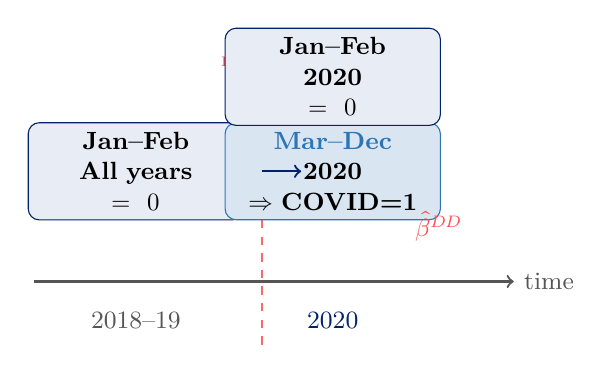
\begin{tikzpicture}[
          box/.style={rectangle, rounded corners=4pt, draw=navyblue,
                      fill=lightbg, font=\small\bfseries,
                      text width=2.5cm, align=center, minimum height=0.85cm},
          hibox/.style={rectangle, rounded corners=4pt,
                        draw=institutgold, fill=institutgold!18,
                        font=\small\bfseries, text width=2.5cm,
                        align=center, minimum height=0.85cm},
          arr/.style={->, thick, navyblue}
        ]
        %% Timeline axis
        \draw[->, thick, medgray] (-0.3, 0) -- (5.8, 0)
              node[right, font=\small] {time};
        %% Year labels
        \node[font=\small, color=medgray] at (1.0, -0.5) {2018--19};
        \node[font=\small, color=navyblue] at (3.5, -0.5) {2020};
        %% Vertical divider (lockdown)
        \draw[thick, dashed, red!60] (2.6, -0.8) -- (2.6, 2.6)
              node[above, font=\tiny, color=red!70] {Lockdown};
        %% Pre box
        \node[box] at (1.0, 1.4) {Jan--Feb\\All years\\$=0$};
        %% Post box
        \node[hibox] at (3.5, 1.4)
              {\gold{Mar--Dec}\\2020\\$\Rightarrow$ COVID=1};
        %% Control months (Jan-Feb 2020)
        \node[box] at (3.5, 2.6) {Jan--Feb\\2020\\$=0$};
        %% Beta arrow
        \draw[arr] (2.6, 1.4) -- (3.1, 1.4);
        \node[font=\small\bfseries, color=red!70] at (4.85, 0.7)
              {$\hat{\beta}^{DD}$};
      \end{tikzpicture}}
      \end{center}
    \end{column}
  \end{columns}
\end{frame}

%% ---- 5. Main Result -----------------------------------------
\begin{frame}{Main Result: Non-Healthcare Institutions Drove the Increase}
  \begin{columns}
    \begin{column}{0.52\textwidth}
      \textbf{Difference-in-Differences results} (Table 2):

      \vspace{0.1em}
      \begin{center}
      \scriptsize
      \begin{tabular}{lccc}
        \toprule
         & \textbf{Overall} & \textbf{Health} & \textbf{Non-Health} \\
        \midrule
        1(COVID-19) & \pos{0.120***} & $-$0.060 & \pos{0.166***} \\
                    & (0.034)         & (0.043)   & (0.039) \\
        $N$         & 2,304           & 468       & 1,836 \\
        $R^2$       & 0.32            & 0.19      & 0.35 \\
        Pre-COVID mean & 0.705        & 0.667     & 0.715 \\
        \% change   & \pos{$+$17.02\%} & $-$9.09\% & \pos{$+$23.21\%} \\
        \bottomrule
      \end{tabular}
      \end{center}

      \vspace{0.2em}
      {\small \color{medgray}
        *** $p<0.01$. Baseline FE at institution, month, and year level.
        Source: IMCO.}
    \end{column}
    \begin{column}{0.44\textwidth}
      \begin{resultbox}
        \textbf{The counterintuitive result:}\\[0.2em]
        The pandemic increased discretionary contracting by
        \gold{$+$17\%} overall.\\[0.15em]
        This is driven entirely by
        \gold{non-healthcare institutions ($+$23\%).}\\[0.15em]
        Healthcare institutions show \bad{no significant change},
        despite being at the center of the public debate.
      \end{resultbox}

      \begin{keybox}
        A possible explanation: intense media scrutiny of healthcare
        procurement may have \navy{constrained discretionary behavior}
        precisely where it was most expected.
      \end{keybox}
    \end{column}
  \end{columns}
\end{frame}

%% ---- 6. Event Study & Mechanisms ----------------------------
\begin{frame}{Dynamic Effects and Mechanisms}
  \begin{columns}
    \begin{column}{0.50\textwidth}
      \textbf{Event study (Figure 1):}

      \begin{center}
        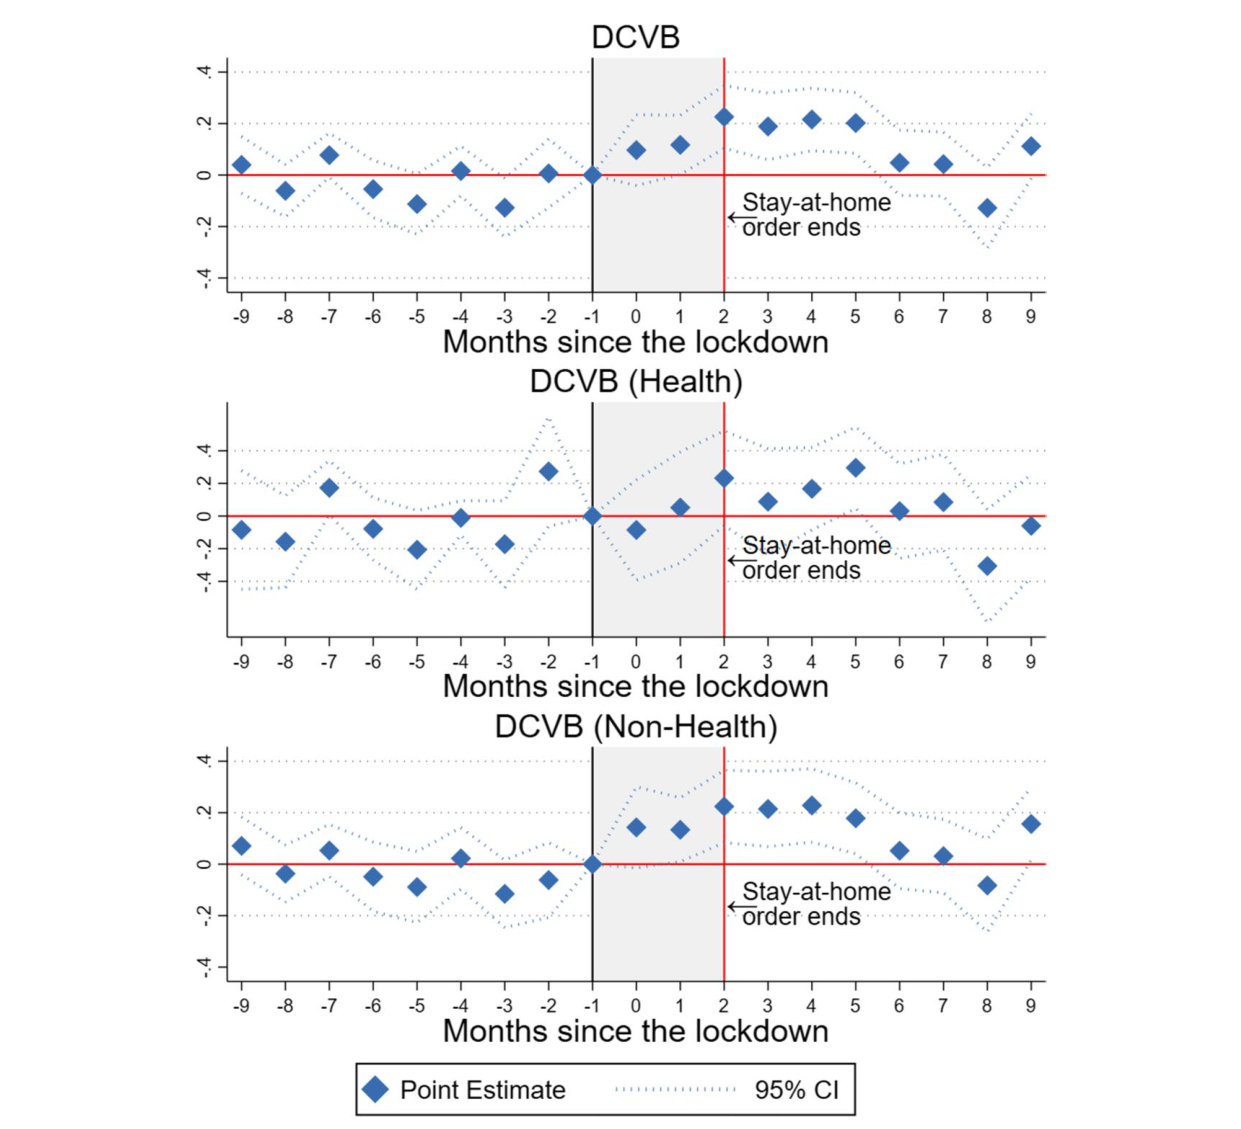
\includegraphics[width=0.70\linewidth]{../Figures/figure1_event_study_p04.png}
      \end{center}

      {\small \color{medgray}
        Pre-pandemic coefficients near zero (parallel trends).
        Non-health DCVB peaks at $q=2$ (May 2020), fades within 6 months.
        Healthcare DCVB flat throughout.}
    \end{column}
    \begin{column}{0.46\textwidth}
      \textbf{Two mechanisms investigated:}

      \vspace{0.35em}
      \textbf{\small Market concentration (HHI):}\\[0.15em]
      {\small Each institution's supplier market is measured with a
      Herfindahl-Hirschman Index. Non-healthcare institutions saw their
      supplier market become significantly more concentrated.}

      \vspace{0.35em}
      \textbf{\small Late disclosure of contract information:}\\[0.15em]
      {\small The proportion of contracts with procedural information
      published after the contract start date increased for non-healthcare
      institutions, consistent with reduced transparency.}

      \vspace{0.3em}
      {\small \color{medgray}
        Leave-one-out analysis and exclusion of SEDENA confirm robustness.}
    \end{column}
  \end{columns}
\end{frame}

%% ---- 7. Conclusions -----------------------------------------
\begin{frame}{Conclusions and Policy Implications}
  \begin{columns}
    \begin{column}{0.54\textwidth}
      \textbf{What we found:}
      \begin{itemize}
        \item COVID-19 increased discretionary contracting in Mexico's
              federal procurement by \gold{$+$17\%} on average
        \item The effect is driven entirely by
              \gold{non-healthcare institutions ($+$23\%),}
              not by healthcare
        \item The increase was \gold{temporary:} peaked two months after
              the stay-at-home order was lifted, returned to baseline
              within six months
        \item Non-healthcare institutions simultaneously became more
              \gold{concentrated} in their supplier base and less
              \gold{transparent} in contract disclosure
      \end{itemize}

      \vspace{0.2em}
      {\small \textbf{Limitation:} DCVB measures \emph{corruption risk},
      not actual corruption. The paper identifies a pattern at the
      aggregate level, not individual wrongdoing.}
    \end{column}
    \begin{column}{0.42\textwidth}
      \begin{resultbox}
        \textbf{Policy implication:}\\[0.5em]
        Audit efforts targeting pandemic-era procurement should focus on
        \gold{non-healthcare institutions,} even though the political
        debate centered on healthcare.\\[0.5em]
        Public scrutiny may itself be a \navy{corruption deterrent:}
        sectors that receive less attention are where the risk
        actually materializes.
      \end{resultbox}

      \vspace{0.2em}
      {\small \color{medgray}
        Silverio-Murillo, Prudencio \& Balmori-de-la-Miyar (2024),
        \textit{Public Organization Review} 24, 1293--1313.}
    \end{column}
  \end{columns}
\end{frame}

\end{document}
